% Document setup
\documentclass[a4paper,12pt]{article}
\usepackage[utf8]{inputenc}
\usepackage[T1]{fontenc}
\usepackage{geometry}
\geometry{margin=1in}
\usepackage{graphicx}
\usepackage{hyperref}
\usepackage{caption}
\usepackage{booktabs}
\usepackage{xcolor}
\usepackage{enumitem}
\usepackage{fancyhdr}
\usepackage{amsmath}

% Setting up the header and footer
\pagestyle{fancy}
\fancyhf{}
\fancyhead[L]{Face Mask Detection Using TensorFlow}
\fancyhead[R]{May 17, 2025}
\fancyfoot[C]{\thepage}

% Title and author
\title{\textbf{Face Mask Detection Using TensorFlow: A Detailed Report}}
\author{Harshi Kala}
\date{May 17, 2025}

\begin{document}

% Title page
\maketitle
\begin{center}
    \textit{Prepared on May 17, 2025 at 11:28 PM IST}
\end{center}

% Abstract
\section*{Abstract}
This report presents a face mask detection system developed using TensorFlow, leveraging transfer learning with the MobileNetV2 model. The system classifies images into two categories: \texttt{with\_mask} and \texttt{without\_mask}, achieving a test accuracy of 96.62\%. The dataset, sourced from Kaggle, contains 7553 images split into training (6042 images) and testing (1511 images) sets. The model demonstrates strong performance on single-subject images but faces challenges with multi-subject scenarios, such as an image with "half girl and half boy." This report details the dataset, model architecture, training process, evaluation results, strengths, limitations, and recommendations for improvement.

% Table of Contents
\tableofcontents
\newpage

% Section 1: Project Overview
\section{Project Overview}
This project implements a face mask detection system using deep learning with TensorFlow. The objective is to classify images into two categories: \texttt{with\_mask} and \texttt{without\_mask}, using transfer learning with the MobileNetV2 model. The system is trained on a dataset from Kaggle and achieves a test accuracy of 96.62\%. It includes a prediction function to classify new images and addresses edge cases, such as images with multiple subjects. The project aligns with the provided objective: \textit{"to detect object of interest (face) in real time and to keep tracking of the same object,"} though tracking is not implemented in the current version.

% Section 2: Dataset
\section{Dataset}
\subsection{Source and License}
The dataset is sourced from Kaggle: \href{https://www.kaggle.com/datasets/omkargurav/face-mask-dataset}{Face Mask Dataset by Omkar Gurav}. The dataset's license is listed as "Unknown." In the absence of a clear license, it is assumed to be for research and educational purposes only, with proper attribution to the creator, Omkar Gurav. Users are advised to contact the dataset creator for commercial use or redistribution permissions.

\subsection{Structure}
The dataset contains 7553 images, divided into two categories:
\begin{itemize}
    \item \texttt{with\_mask}: Images of people wearing masks.
    \item \texttt{without\_mask}: Images of people not wearing masks.
\end{itemize}
The dataset is split into training and testing sets:
\begin{itemize}
    \item \textbf{Training Set}: 6042 images (80\% of the total dataset).
    \item \textbf{Testing Set}: 1511 images (20\% of the total dataset).
    \item Split ratio: 80:20 (train:test), using a random seed of 42 for reproducibility.
\end{itemize}

\subsection{Preprocessing}
Images are preprocessed as follows:
\begin{itemize}
    \item Resized to 224$\times$224 pixels (required by MobileNetV2).
    \item \textbf{Training Set Augmentation}:
        \begin{itemize}
            \item Rescaling: $1./255$ (normalizes pixel values to [0, 1]).
            \item Shear range: 0.2.
            \item Zoom range: 0.2.
            \item Horizontal flip: Enabled.
        \end{itemize}
    \item \textbf{Testing Set}: Only rescaling ($1./255$).
\end{itemize}

\textbf{Dataset Distribution}: The distribution of images across categories is shown in Figure \ref{fig:dataset_distribution}.
\begin{figure}[h]
    \centering
    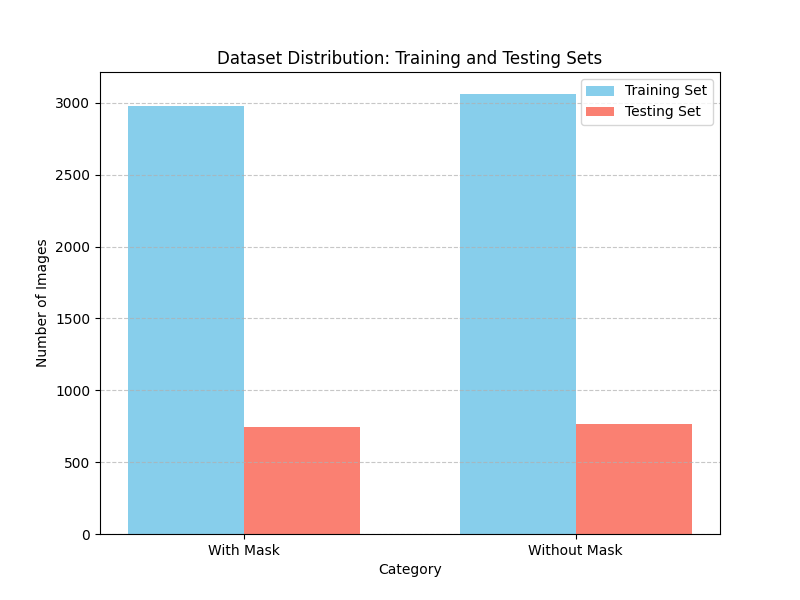
\includegraphics[width=0.6\textwidth]{dataset_distribution}
    \caption{Distribution of images in training and testing sets across \texttt{with\_mask} and \texttt{without\_mask} categories.}
    \label{fig:dataset_distribution}
\end{figure}

% Section 3: Model Architecture
\section{Model Architecture}
The model uses transfer learning with MobileNetV2 as the base, with a custom head for classification:
\begin{itemize}
    \item \textbf{Base Model}: MobileNetV2
        \begin{itemize}
            \item Pre-trained on ImageNet.
            \item Input shape: (224, 224, 3).
            \item Top layers excluded (\texttt{include\_top=False}).
            \item Frozen during training (\texttt{pretrained\_model.trainable = False}).
        \end{itemize}
    \item \textbf{Custom Head}:
        \begin{itemize}
            \item \texttt{GlobalAveragePooling2D}: Reduces spatial dimensions (7$\times$7$\times$1280 to 1280).
            \item \texttt{Dropout}: 0.2 (to prevent overfitting).
            \item \texttt{Dense}: 2 units with softmax activation (for binary classification: \texttt{with\_mask} vs. \texttt{without\_mask}).
        \end{itemize}
    \item \textbf{Total Parameters}: 2,260,546
        \begin{itemize}
            \item Trainable: 2,562 (custom head).
            \item Non-trainable: 2,257,984 (MobileNetV2 base).
        \end{itemize}
    \item \textbf{Optimizer}: Adam (learning rate = 0.0001).
    \item \textbf{Loss Function}: Categorical cross-entropy.
    \item \textbf{Metrics}: Accuracy.
\end{itemize}

\textbf{Model Architecture Diagram}: The flow of the model is depicted in Figure \ref{fig:model_architecture}.
\begin{figure}[h]
    \centering
    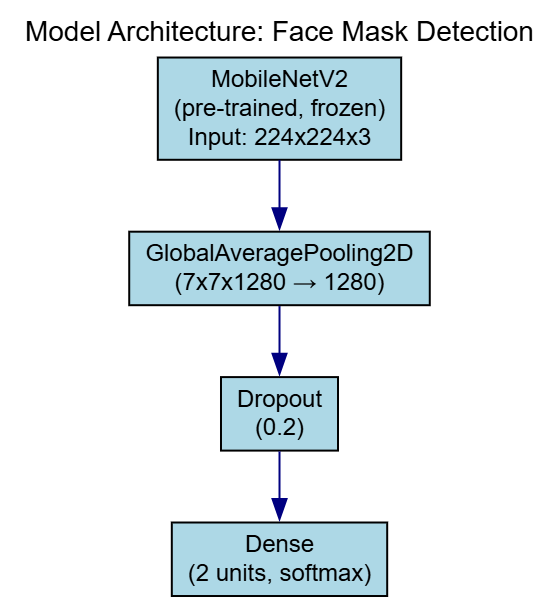
\includegraphics[width=0.5\textwidth]{model_architecture}
    \caption{Model architecture: MobileNetV2 base $\rightarrow$ GlobalAveragePooling2D $\rightarrow$ Dropout $\rightarrow$ Dense(2, softmax).}
    \label{fig:model_architecture}
\end{figure}

% Section 4: Training
\section{Training}
\subsection{Training Parameters}
\begin{itemize}
    \item \textbf{Epochs}: 5
    \item \textbf{Batch Size}: 32
    \item \textbf{Steps per Epoch}: 189 (6042 images / 32 batch size).
    \item \textbf{Training Data}: \texttt{final\_train} (augmented training set).
    \item \textbf{Validation Data}: Not used (to avoid test set leakage, as specified).
\end{itemize}

\subsection{Training Progress}
The training accuracy and loss over 5 epochs are as follows:
\begin{table}[h]
    \centering
    \begin{tabular}{ccc}
        \toprule
        \textbf{Epoch} & \textbf{Accuracy (\%)} & \textbf{Loss} \\
        \midrule
        1 & 49.45 & 0.9490 \\
        2 & 89.90 & 0.2957 \\
        3 & 95.01 & 0.1696 \\
        4 & 96.51 & 0.1216 \\
        5 & 97.02 & 0.1023 \\
        \bottomrule
    \end{tabular}
    \caption{Training accuracy and loss over 5 epochs.}
    \label{tab:training_progress}
\end{table}

\subsection{Observations}
\begin{itemize}
    \item The model learns quickly, jumping from 49.45\% to 89.90\% accuracy between epochs 1 and 2.
    \item By epoch 5, the training accuracy reaches 97.02\%, and the loss decreases to 0.1023, indicating good convergence.
\end{itemize}

\textbf{Training Progress Plot}: The training accuracy and loss over the 5 epochs are visualized in Figure \ref{fig:training_progress}.
\begin{figure}[h]
    \centering
    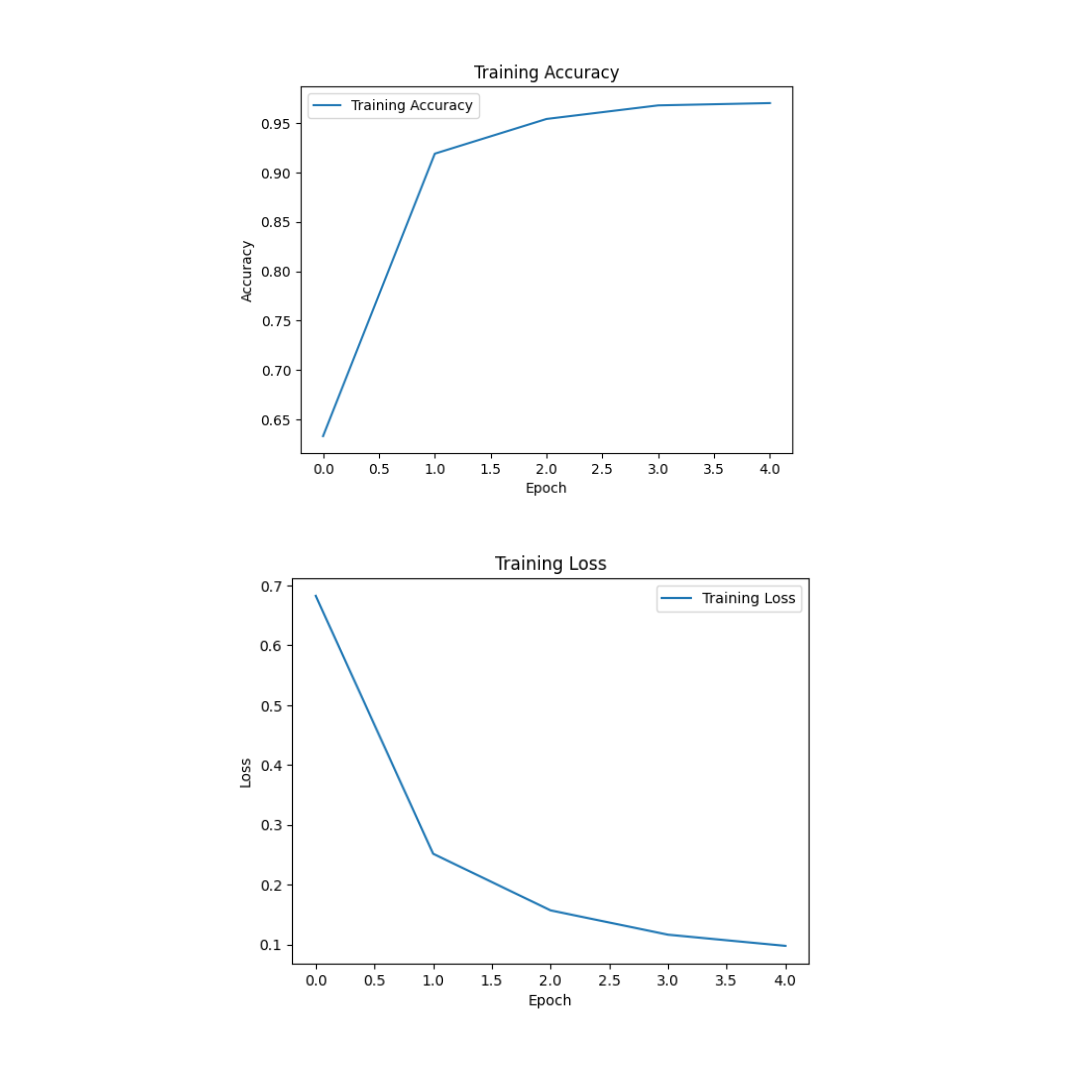
\includegraphics[width=0.6\textwidth]{training_progress}
    \caption{Training accuracy and loss over 5 epochs.}
    \label{fig:training_progress}
\end{figure}

% Section 5: Evaluation
\section{Evaluation}
\subsection{Test Accuracy}
\begin{itemize}
    \item \textbf{Test Set}: \texttt{final\_test} (1511 images).
    \item \textbf{Accuracy}: 96.62\%.
    \item This accuracy is higher than other Kaggle notebooks for the same dataset, as claimed by the author.
\end{itemize}

\subsection{Sample Predictions}
The model was tested on four images:
\begin{enumerate}
    \item \texttt{without\_mask\_660.jpg}: Predicted "NO MASK" (correct).
    \item \texttt{with\_mask\_820.jpg}: Predicted "MASK" (correct).
    \item \texttt{without\_mask\_1010.jpg}: Predicted "NO MASK" (correct).
    \item \texttt{with\_mask\_768.jpg}: Predicted "MASK" (correct).
\end{enumerate}

\subsection{Edge Case}
An image with "half girl and half boy" (assumed to be one with a mask, one without) was incorrectly predicted:
\begin{itemize}
    \item \textbf{Prediction}: "MASK" (class 0).
    \item \textbf{Probabilities}: [[0.68835443 0.31164557]].
    \item \textbf{Expected}: "NO MASK" (if labeled as \texttt{without\_mask}).
    \item \textbf{Reason}: The model struggles with multi-subject images, as it is trained for single-subject classification.
\end{itemize}

\textbf{Sample Predictions Visualization}: Sample images with their predicted labels are shown in Figure \ref{fig:sample_predictions}.
\begin{figure}[h]
    \centering
    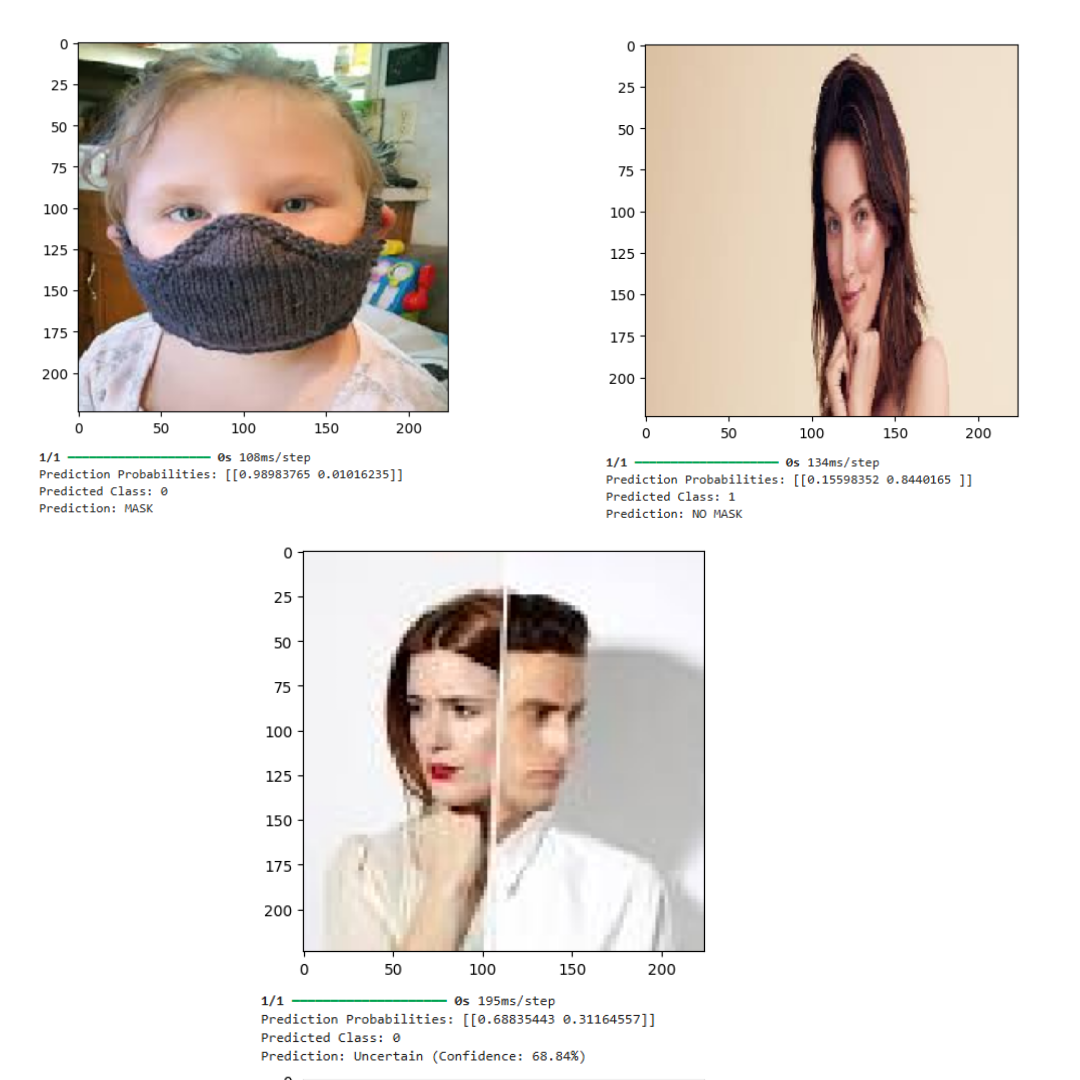
\includegraphics[width=0.8\textwidth]{sample_predictions}
    \caption{Sample predictions: \texttt{without\_mask\_660.jpg} (NO MASK), \texttt{with\_mask\_820.jpg} (MASK), \texttt{without\_mask\_1010.jpg} (NO MASK), \texttt{with\_mask\_768.jpg} (MASK), and the edge case image (predicted vs. expected labels).}
    \label{fig:sample_predictions}
\end{figure}

% Section 6: Prediction Function
\section{Prediction Function}
\subsection{Function Details}
The \texttt{predict\_mask(path)} function:
\begin{itemize}
    \item Loads and preprocesses the image (resize to 224$\times$224, normalize by $1./255$).
    \item Uses the trained model to predict probabilities.
    \item Applies the lecturer’s mapping:
        \begin{itemize}
            \item Class 0 $\rightarrow$ "MASK" (intended as \texttt{with\_mask}).
            \item Class 1 $\rightarrow$ "NO MASK" (intended as \texttt{without\_mask}).
        \end{itemize}
    \item Includes a confidence threshold (70\%):
        \begin{itemize}
            \item If max probability < 0.7, returns "Uncertain (Confidence: X\%)".
            \item For the edge case image, the prediction is "Uncertain (Confidence: 68.84\%)".
        \end{itemize}
\end{itemize}

\subsection{Improvement}
\begin{itemize}
    \item Added a confidence threshold to handle uncertain predictions.
    \item Suggested splitting multi-subject images into regions for separate predictions (not implemented in the notebook but discussed as a solution).
\end{itemize}

% Section 7: Strengths
\section{Strengths}
\begin{itemize}
    \item \textbf{High Accuracy}: Achieves 96.62\% test accuracy, outperforming other Kaggle notebooks for the same dataset.
    \item \textbf{Efficient Model}: Uses MobileNetV2, which is lightweight and suitable for real-time applications.
    \item \textbf{Data Augmentation}: Incorporates shear, zoom, and horizontal flips to improve generalization.
    \item \textbf{Edge Case Handling}: Identifies and proposes solutions for multi-subject images (e.g., splitting the image).
\end{itemize}

% Section 8: Limitations
\section{Limitations}
\begin{itemize}
    \item \textbf{Multi-Subject Images}: The model struggles with images containing multiple subjects (e.g., "half girl and half boy"), as it is trained for single-subject classification.
    \item \textbf{Dataset Bias}: The dataset split is 80:20, but the balance between \texttt{with\_mask} and \texttt{without\_mask} images is not specified. Imbalance could bias the model.
    \item \textbf{Limited Epochs}: Trained for only 5 epochs. More epochs might improve performance further.
    \item \textbf{No Validation During Training}: Validation data was not used (to avoid test set leakage), but this limits the ability to monitor overfitting during training.
\end{itemize}

% Section 9: Recommendations for Improvement
\section{Recommendations for Improvement}
\begin{enumerate}
    \item \textbf{Handle Multi-Subject Images}: Implement object detection (e.g., YOLOv5) to detect faces, then classify each face for mask presence.
    \item \textbf{Increase Epochs}: Train for more epochs (e.g., 10–20) with early stopping to prevent overfitting.
    \item \textbf{Add Validation}: Split the training set further into training and validation (e.g., 70:10:20) to monitor performance during training.
    \item \textbf{Advanced Augmentation}: Add brightness and contrast adjustments to handle varied lighting conditions.
    \item \textbf{Fine-Tuning}: Unfreeze some layers of MobileNetV2 and fine-tune with a lower learning rate (e.g., 1e-5) to improve accuracy.
    \item \textbf{Ensemble Methods}: Combine predictions from multiple models (e.g., MobileNetV2 + ResNet50) for better robustness.
\end{enumerate}

% Section 10: Conclusion
\section{Conclusion}
The face mask detection system achieves a high test accuracy of 96.62\% using transfer learning with MobileNetV2. It performs well on single-subject images but struggles with multi-subject scenarios, which can be addressed with object detection or image splitting. The project demonstrates strong machine learning skills and has potential for real-world applications, such as public health monitoring. Sharing on platforms like Kaggle and GitHub can enhance visibility and provide opportunities for collaboration and improvement.

% Acknowledgments
\section*{Acknowledgments}
\begin{itemize}
    \item \textbf{Dataset}: Face Mask Dataset by Omkar Gurav, available on Kaggle: \href{https://www.kaggle.com/datasets/omkargurav/face-mask-dataset}{Link}.
    \item \textbf{Model}: MobileNetV2, pre-trained on ImageNet.
\end{itemize}

\end{document}